\subsection*{Coeficiente de correlación de Pearson}
Dadas X e Y variables aleatorias, el coeficiente de correlación de Pearson entre X e Y está definido como:

\begin{minipage}{\linewidth}
  \centering
  \begin{minipage}{0.45\linewidth}
    $$\rho_{_{X,Y}} = \frac{Cov(X, Y)}{\sqrt{Var(X) \cdot Var(Y)}}$$
  \end{minipage}
  \hspace{0.05\linewidth}
  \begin{minipage}{0.45\linewidth}
    $$-1 \leq \rho_{_{X,Y}} \leq 1$$
  \end{minipage}
\end{minipage}

Siendo:
$$Cov(X,Y) \dot{=} E[(X - E[X]) \cdot (Y - E[Y])]$$

Dado que no conocemos la distribución de las variables, necesitamos una estimación de $\rho_{_{X,Y}}$. Por lo que utilizaremos:

$$\hat{\rho}_{_{X,Y}} = \frac{\sum\limits_{i=1}^{n} (x_i - \bar{x})(y_i - \bar{y})} {\sqrt{\sum\limits_{i=1}^{n}(x_i - \bar{x})^2} \sqrt{\sum\limits_{i=1}^{n}(y_i - \bar{y})^2}}$$
donde, $\bar{x}$ es el promedio de los valores observados. Y se utiliza el estimador de máxima verosimilitud para el desvío.

\subsection*{Modelo $\Omega$}
Se tienen $n$ observaciones del vector aleatorio $(X_{1}, X_{2}, ..., X_{p-1}, Y)$, se propone, bajo los supuestos necesarios, el siguiente modelo:
$$Y = \beta_{0} + \beta_{1} \cdot x_{1} + ... + \beta_{p-1} \cdot x_{p-1} + \epsilon$$
De forma que, para cada observación se tiene:
$$y_i = \beta_{0} + \beta_{1} \cdot x_{i,1} + ... + \beta_{p-1} \cdot x_{i, p-1} + \epsilon_{i} \quad  \forall i = 1,..,n$$
Con $\epsilon_{i}$ variables aleatorias no observables.\\

\textbf{Supuestos}
\begin{enumerate}
    \item $E[\epsilon_{i}] = 0$
    \item $Var(\epsilon_{i}) = \sigma^2$
    \item $\epsilon_{i} \stackrel{iid}{\sim} \mathcal{N}(0, \sigma^2)$
\end{enumerate}

\textbf{Expresiones}
De ahora en adelante $X$ será fijo en $x$.

\begin{minipage}{\linewidth}
  \centering
  \begin{minipage}{0.10\linewidth}
        \begin{align*}
            Y &= \begin{bmatrix}
            y_{1} \\
            y_{2} \\
            \vdots \\
            y_{n}
            \end{bmatrix}
        \end{align*}
  \end{minipage}
  \hspace{0.05\linewidth}
  \begin{minipage}{0.10\linewidth}
        \begin{align*}
            \epsilon &= \begin{bmatrix}
            \epsilon_{1} \\
            \epsilon_{2} \\
            \vdots \\
            \epsilon_{n}
            \end{bmatrix}
        \end{align*}
  \end{minipage}
  \hspace{0.05\linewidth}
  \begin{minipage}{0.10\linewidth}
        \begin{align*}
            \beta &= \begin{bmatrix}
            \beta_{0} \\
            \beta_{1} \\
            \vdots \\
            \beta_{p-1}
            \end{bmatrix}
        \end{align*}
  \end{minipage}
  \hspace{0.05\linewidth}
  \begin{minipage}{0.40\linewidth}
        \begin{align*}
            \mathbb X &= \begin{bmatrix}
            1 & x_{1,1}  & \dots & x_{1, p-1} \\
            1 & x_{2,1}  & \dots & x_{2, p-1} \\
            \vdots & \vdots & \ddots & \vdots \\
            1 & x_{n,1} & \dots & x_{n, p-1} \\
            \end{bmatrix}
        \end{align*}
  \end{minipage}
\end{minipage}
\vskip0.5cm
Por lo tanto, se tiene que:
$$Y = \mathbb X \beta + \epsilon$$
Y, si $\mathbb X$ tiene rango completo, entonces se deducen las siguientes expresiones

$$ \hat{\beta} = ({\mathbb X}^T \mathbb X)^{-1} {\mathbb X}^T Y$$
$$ \hat{Y} = \mathbb X ({\mathbb X}^T \mathbb X)^{-1}{\mathbb X}^T Y = P Y$$

Por último, se define como \textbf{residuo} a $r = Y - \hat{Y}$

\subsection*{Test de hipótesis}
Bajo el modelo $\Omega$: los estimadores $\hat{\beta}$ y $S^{2}$ son IMVU (\textbf{I}nsesgado de \textbf{M}ínima \textbf{V}arianza \textbf{U}niformemente)

\vskip0.4cm
\textbf{Test t}
\vskip0.2cm
\begin{minipage}{\linewidth}
  \begin{minipage}{0.40\linewidth}
    \centering
    $H_0: \beta_{i} = 0$
  \end{minipage}
  \hspace{0.05\linewidth}
  \begin{minipage}{0.05\linewidth}
    \centering vs
  \end{minipage}
  \hspace{0.05\linewidth}
  \begin{minipage}{0.40\linewidth}
    \centering
    $H_1: \beta_{i} \neq 0$
  \end{minipage}
\end{minipage}
\vskip0.2cm
Sabiendo que $\hat{\beta_{i}} \sim \mathcal{N}(\beta_{i}, \sigma^2 D_{i,i})$ se obtiene el estadístico $T$ de la siguiente forma:
$$
T = \frac{\hat{\beta_{i}} - \beta_{i}}{S \sqrt{D_{i,i}}}
$$
siendo $D_{i,i}$ el elemento $i$ de la diagonal de la matriz $({\mathbb X}^{T} \mathbb X)^{-1}$\\
\vskip0.2cm
\begin{minipage}{\linewidth}
  \begin{minipage}{0.55\linewidth}
    \begin{figure}[H]
        \centering
        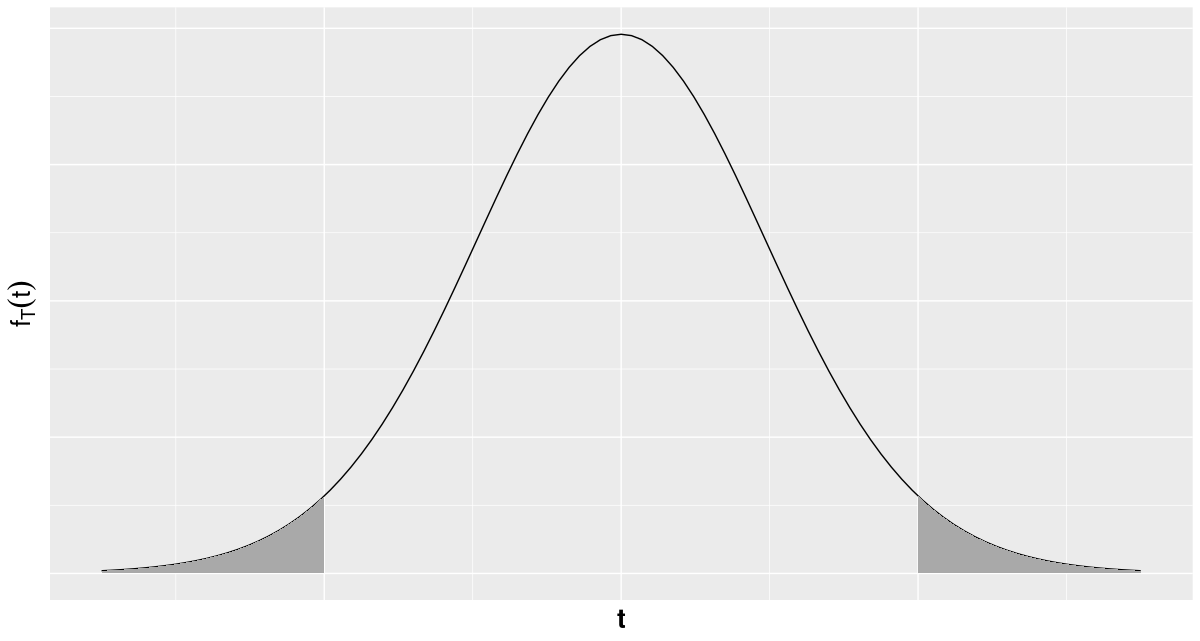
\includegraphics[width=1\textwidth]{resources/t_student_density.png}
        \caption{Densidad de T bajo $H_0$}
    \end{figure}
  \end{minipage}
  \hspace{0.05\linewidth}
  \begin{minipage}{0.35\linewidth}
        De forma que bajo $H_0$ se tiene que 
        $$T \sim t_{n-p}$$
        Por lo que, se calculará el p-valor como el area sombreada en la figura
        $$ p-value = P(|T| > t_{obs})$$
  \end{minipage}
\end{minipage}
\vskip0.4cm
\textbf{Test F}
\vskip0.2cm
\begin{minipage}{\linewidth}
  \begin{minipage}{0.40\linewidth}
    \centering
    $H_0: \beta_{1} = ... = \beta_{p-1} = 0$
  \end{minipage}
  \hspace{0.05\linewidth}
  \begin{minipage}{0.05\linewidth}
    \centering vs
  \end{minipage}
  \hspace{0.05\linewidth}
  \begin{minipage}{0.40\linewidth}
    \centering
    $H_1:$ Algún $\beta_{i} \neq 0$
  \end{minipage}
\end{minipage}
\vskip0.2cm

El estadístico a utilizar para este Test será $F$, cuya expresión será la siguiente
$$
F = \frac{(C\hat{\beta})^{T} (C ({\mathbb X}^T \mathbb X)^{-1} {C}^{T})^{-1}(C \hat{\beta})}{(p-1) S^{2}} \stackrel{H_0}{\sim} {\mathcal F}_{p-1, n-p}
$$
siendo
\begin{align*}
    C &= \begin{bmatrix}
    0 & 1 & 0 & \dots & 0 \\
    0 & 0 & 1 & \dots & 0 \\
    \vdots & \vdots & \vdots & \ddots & \vdots \\
    0 & 0 & 0 & \dots & 1 \\
    \end{bmatrix} \in \mathbb R ^{(p-1) \times p}, \quad rg(C) = p-1
\end{align*}

\vskip0.2cm
\begin{minipage}{\linewidth}
  \begin{minipage}{0.55\linewidth}
    \begin{figure}[H]
        \centering
        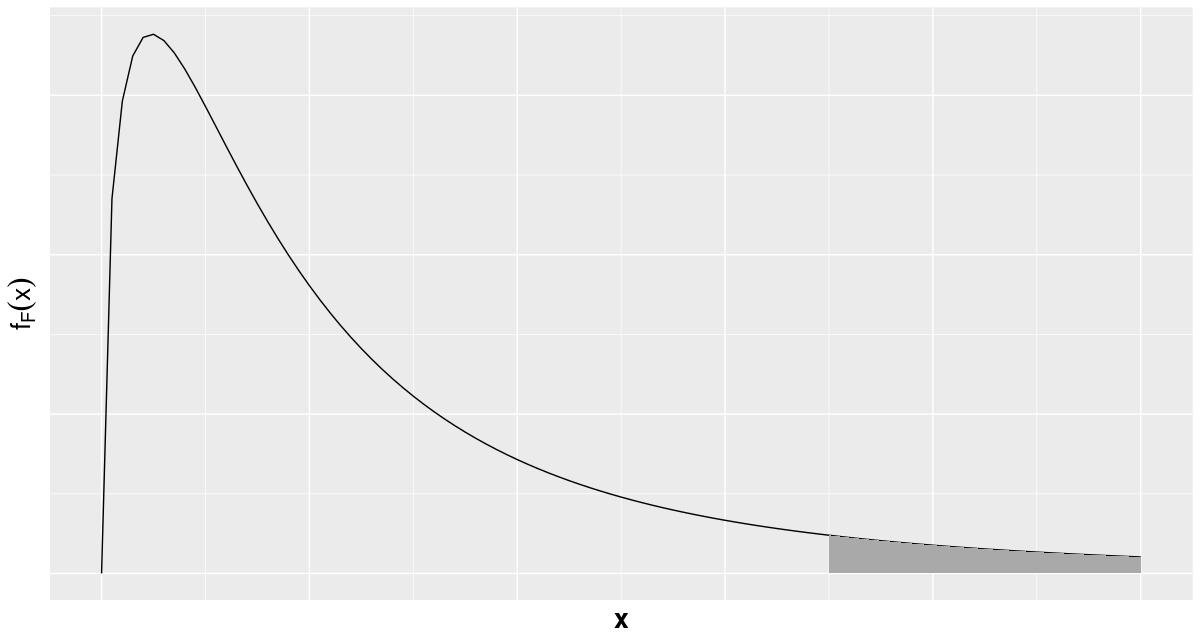
\includegraphics[width=1\textwidth]{resources/f_fisher_density.png}
        \caption{Densidad de F bajo $H_0$}
    \end{figure}
  \end{minipage}
  \hspace{0.05\linewidth}
  \begin{minipage}{0.35\linewidth}
        Por lo que, se calculará el p-valor como el area sombreada en la figura
        $$ p-value = P(F > x_{obs})$$
  \end{minipage}
\end{minipage}
\vskip0.4cm
\textbf{Observación:} a lo largo del trabajo práctico tomaremos un nivel de significancia mínimo $\alpha = 0.05$ de forma que para cualquier p-valor menor a $\alpha$ rechazaremos siempre la hipótesis nula.

\subsection*{Selección de variables}
En el trabajo práctico utilizaremos el método de selección \textbf{StepWise: forward} una heurística greedy que analiza los modelos desde el más simple (sólo 1 variable predictora) hasta el más complejo (todas las variables predictoras) de forma incremental. Su método de selección se basa en el test F: irá seleccionando las variables predictoras en base al modelo que obtenga un estadístico F mayor.

\subsection*{Análisis de residuos}
Los residuos, previamente definidos como $r_i = y_i - \hat{y}_{i}$ serán variables aleatorias con:
\begin{center}
    \begin{itemize}
        \item $E[r_i] = 0$
        \item $Var[r_i] = {\sigma}^2(1-P_{i,i})$
    \end{itemize}
\end{center}
Asumiendo que siguen una distribución normal se tiene que:
$$
\frac{r_i}{\sqrt{\sigma^2 (1-P_{i,i})}} \sim \mathcal{N}(0, 1)
$$
Pero como desconocemos el valor de $\sigma^2$ se utilizarán los \textbf{residuos studentizados}, que se definen de la siguiente manera:
$$
t_i = \frac{r_i}{\sqrt{S^2(1-P_{i,i})}}
$$
tal que si $r_i$ llevan una distribución normal los $t_i$ tendrán distribución t-student.
\vskip0.2cm\textbf{Comparación según error cuadrático medio}\\
Para realizar comparaciones basadas en el ECM (Error Cuadrático Medio) que no subestimen el valor obtenido se utilizarán los residuos de LOOCV (Leave One Out Cross Validation), que consisten en, para un mismo modelo, realizar la regresión para todas las observaciones en la muestra menos 1.\\
Se definen entonces los residuos de validación cruzada como:
$$
r_{-i} =  = y_{i} - \hat{\beta}_{-i} x_i
$$
siendo $\hat{\beta}_{-i}$ los coeficientes obtenidos de la regresión sin tener en cuenta la observación $i$.\\
Este residuo se calculará de manera equivalente con la siguiente expresión:
$$
r_{-i} = \frac{r_i}{1-P_{i,i}}
$$
Y se definirá en base a este último lo que llamaremos $ECM_{VC}$ (Error cuadrático medio de validación cruzada)
$$
EMC_{VC} = \frac{1}{n} \sum^{n}_{i=1}(r_{-i})^2
$$